\documentclass[10pt]{article}

% Pacotes extras necessários
\usepackage{amsmath}
\usepackage[lmargin=0.5in, rmargin=0.5in, tmargin=0.5in, bmargin=0.5in, includehead, includefoot]{geometry}
\usepackage{amsfonts}
\usepackage[utf8]{inputenc}
\usepackage[portuguese]{babel}
\usepackage{graphicx}
\usepackage{fancyhdr}
\usepackage{setspace}
\usepackage{listings}
\usepackage{url}
\usepackage{enumitem}
\usepackage{appendix} % For creating appendix sections
\usepackage{subcaption} % Use subcaption para legendas modernas

% More defined colors
\usepackage[dvipsnames]{xcolor}

% Define a custom style for the code listing
\lstdefinestyle{mystyle}{
    language=Matlab,
    inputencoding=latin1,
    extendedchars=true,
    backgroundcolor=\color{white},   % Choose the background color
    basicstyle=\ttfamily\footnotesize, % Set the font and size for the code
    numbers=left,                    % Line numbers on the left
    numberstyle=\tiny\color{gray},   % Line numbers style
    numbersep=5pt,                   % Distance of line numbers from the code
    tabsize=2,                       % Set tab size (default is 8 spaces)
    breaklines=true,                 % Automatically wrap long lines
    keywordstyle=\color{blue},       % Keywords in blue
    commentstyle=\color{green!60!black}, % Comments in green
    stringstyle=\color{orange},      % Strings in orange
    frame=single,                    % Draw a frame around the code
    keepspaces=true,                 % Preserve spaces in text
    showspaces=false,                % Don't show spaces in strings
    showstringspaces=false,          % Don't show spaces in strings
    showtabs=false,                  % Don't show tabs in strings
    % Add any other options you need
}

\lstset{style=mystyle} % Set the custom style
 
% Required package
\usepackage{tikz}
\usetikzlibrary{positioning}

\graphicspath{ {./images/} }

% Sets para outras partes
\setlength{\parindent}{0pt}
\setstretch{1.5}
\DeclareMathOperator{\sen}{sen}
\DeclareMathOperator{\sinc}{sinc}

%% Facilidades
%% -- Laplace
\newcommand{\Lap}[1]{\mathcal{L}\left\{#1\right\}}

%% -- Negrito em matemáticas
\newcommand{\bm}[1]{\boldsymbol{#1}}


% ------- Estilo do trabalho -------- %
\fancypagestyle{capa}{
    \fancyhf{}
    \renewcommand\headrulewidth{0pt}
}

\pagestyle{fancy}
\fancyhead{}
\fancyhead[L]{\thepage}
\fancyfoot{}
% ----------------------------------- %

% Dados do Grupo
\title{ Robótica e Automação - Trabalho Nº1}
\author{
    Leonardo Soares da Costa Tanaka - DRE: 121067652 \\
    Engenharia de Controle e Automação/UFRJ \\
    Rio de Janeiro, Brasil \\
    Novembro de 2024
}
\date{}

\begin{document}
\maketitle
\thispagestyle{capa}

\section{Introdução}

\quad Este trabalho tem como objetivo explorar a modelagem cinemática de um sistema robótico composto por um braço robótico Kuka KR90 de 6 graus de liberdade e uma mesa posicionadora KUKA KP2 de 2 graus de liberdade.
O efetuador do braço é uma tocha de soldagem, e a cinemática do sistema é descrita por meio de dois arquivos URDF: um para o braço e outro para a mesa.
Com base nesses arquivos e na transformação homogênea Tat fornecida, será possível determinar os parâmetros de Denavit-Hartenberg (DH) de ambos os subsistemas (KR90 e KP2) e do sistema integrado KR90-KP2, visando descrever a cinemática direta e desenvolver o modelo no Matlab utilizando o toolbox de robótica de Peter Corke.
O trabalho também inclui a validação da cinemática direta e inversa do sistema através de uma trajetória de waypoints pré-definidos, assim como a determinação e validação do Jacobiano do sistema.

\section{Desenvolvimento}

\quad Foi considerado o sistema da figura composto por um braço robótico Kuka KR90 do tipo 6R e uma
mesa posicionadora KUKA KP2 do tipo 2R.

\begin{figure}[h]
    \centering
    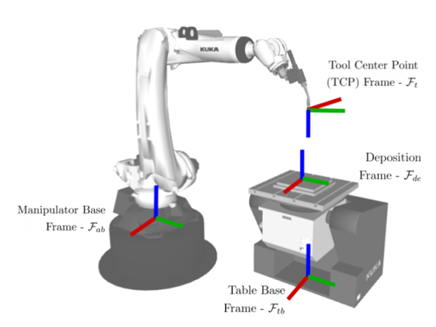
\includegraphics[scale=0.65]{figura1.png}
    \caption{Braço robótico e mesa posicionadora}
\end{figure}

\quad Foi considerado que o efetuador do braço manipulador é uma tocha para soldagem.
Ademais, a cinemática deste sistema robótico é descrito em 2 arquivos urdf, um descrevendo a
cinemática do KR90, kr90.urdf e outro descrevendo a cinemática da mesa posicionadora
KP2, kp2.urdf.
Além disso, foi considerado que a transformação homogênea do sistema de coordenadas da mesa $F_{tb}$ com
respeito a base do braço $F_{ab}$ é dada por:

\begin{equation}
    T_{at} = \begin{bmatrix}
        -1 & 0 & 0 & 1.73923 \\
        0 & -1 & 0 & 0.39198 \\
        0 & 0 & 1 & -0.46360 \\
        0 & 0 & 0 & 1 
        \end{bmatrix}
\end{equation}

\subsection{Parâmetros de Denavit-Hartenberg do braço robótico KR90}

\quad Para determinar os parâmetros de Denavit-Hartenberg do braço robótico KR90, foi necessário analisar o URDF desse braço robótico que pode ser descrito pela seguinte tabela:

\begin{table}[h!]
    \centering
    \begin{tabular}{|c|c|c|c|c|c|c|}
    \hline
    \textbf{Joint $i$} & \textbf{parent} & \textbf{child} & \textbf{xyz} & \textbf{rpy} & \textbf{type} & \textbf{axis} \\ \hline
    1 & kr90\_base\_link & kr90\_link\_1 & 0, 0, 0.675 & 0, 0, 0 & revolute & 0, 0, -1 \\ \hline
    2 & kr90\_link\_1 & kr90\_link\_2 & 0.35, 0, 0 & 0, 0, 0 & revolute & 0, 1, 0 \\ \hline
    3 & kr90\_link\_2 & kr90\_link\_3 & 1.35, 0, 0 & 0, 0, 0 & revolute & 0, 1, 0 \\ \hline
    4 & kr90\_link\_3 & kr90\_link\_4 & 0, 0, -0.041 & 0, 0, 0 & revolute & -1, 0, 0 \\ \hline
    5 & kr90\_link\_4 & kr90\_link\_5 & 1.2, 0, 0 & 0, 0, 0 & revolute & 0, 1, 0 \\ \hline
    6 & kr90\_link\_5 & kr90\_link\_6 & 0.215, 0, 0 & 0, 1.5708, 0 & revolute & 0, 0, -1 \\ \hline
    7 & kr90\_link\_6 & kr90\_tool0 & 0.03046, 0.033, 0.43161 & -0.2356, 0.8988, -0.0942 & fixed & - \\ \hline
    \end{tabular}
    \caption{URDF do braço robótico KR90}
\end{table}

\quad Além disso, foi posicionado o eixo z do sistema de coordenadas 0 \((z_0)\) no mesmo sentido e direção do eixo de rotação da junta 1.
Fazendo a seguinte transformação homogênea da base para o eixo de coordenadas 0:

\begin{equation}
    T_{b0} = \begin{bmatrix}
        1 & 0 & 0 & 0 \\
        0 & -1 & 0 & 0 \\
        0 & 0 & -1 & 0 \\
        0 & 0 & 0 & 1 
        \end{bmatrix}
\end{equation}

\quad Então, foi possível obter os parâmetros do Denavit-Hartenberg Standard a seguir:

\begin{table}[h!]
    \centering
    \begin{tabular}{|c|c|c|c|c|c|c|}
    \hline
    \textbf{Elo $i$} & $\theta_i$ & $d_i$ & $a_i$ & $\alpha_i$ & \textbf{type} & \textbf{offset} \\ \hline
    1 & $\theta_1$ & -0.675 & 0.35 & $\pi/2$ & revolute & 0 \\ \hline
    2 & $\theta_2$ & 0 & 1.35 & 0 & revolute & 0 \\ \hline
    3 & $\theta_3$ & 0 & 0.041 & $-\pi/2$ & revolute & $\pi/2$ \\ \hline
    4 & $\theta_4$ & -1.2 & 0 & $\pi/2$ & revolute & 0 \\ \hline
    5 & $\theta_5$ & 0 & 0 & $-\pi/2$ & revolute & 0 \\ \hline
    6 & $\theta_6$ & -0.215 & 0 & $-\pi$ & revolute & 0 \\ \hline
    \end{tabular}
    \caption{DH do braço robótico}
\end{table}

\quad Além disso, foi necessário obter a transformação homogênea do sistema de coordenadas 6 para o efetuador a seguir:

\begin{equation}
    T_{6e} = \begin{bmatrix}
        0.61978941 & -0.09040281 & 0.77954372 & 0.03046 \\
        -0.05855747 & 0.98524594 & 0.16081497 & 0.033 \\
        -0.78258041 & -0.14531952 & 0.60535125 & 0.43161 \\
        0 & 0 & 0 & 1 
        \end{bmatrix}
\end{equation}

\quad Para obter os parâmetros de Denavit-Hartenberg e as transformações homogêneas acima,
foi seguido os seguintes diagramas:

\begin{figure}[h]
    \centering
    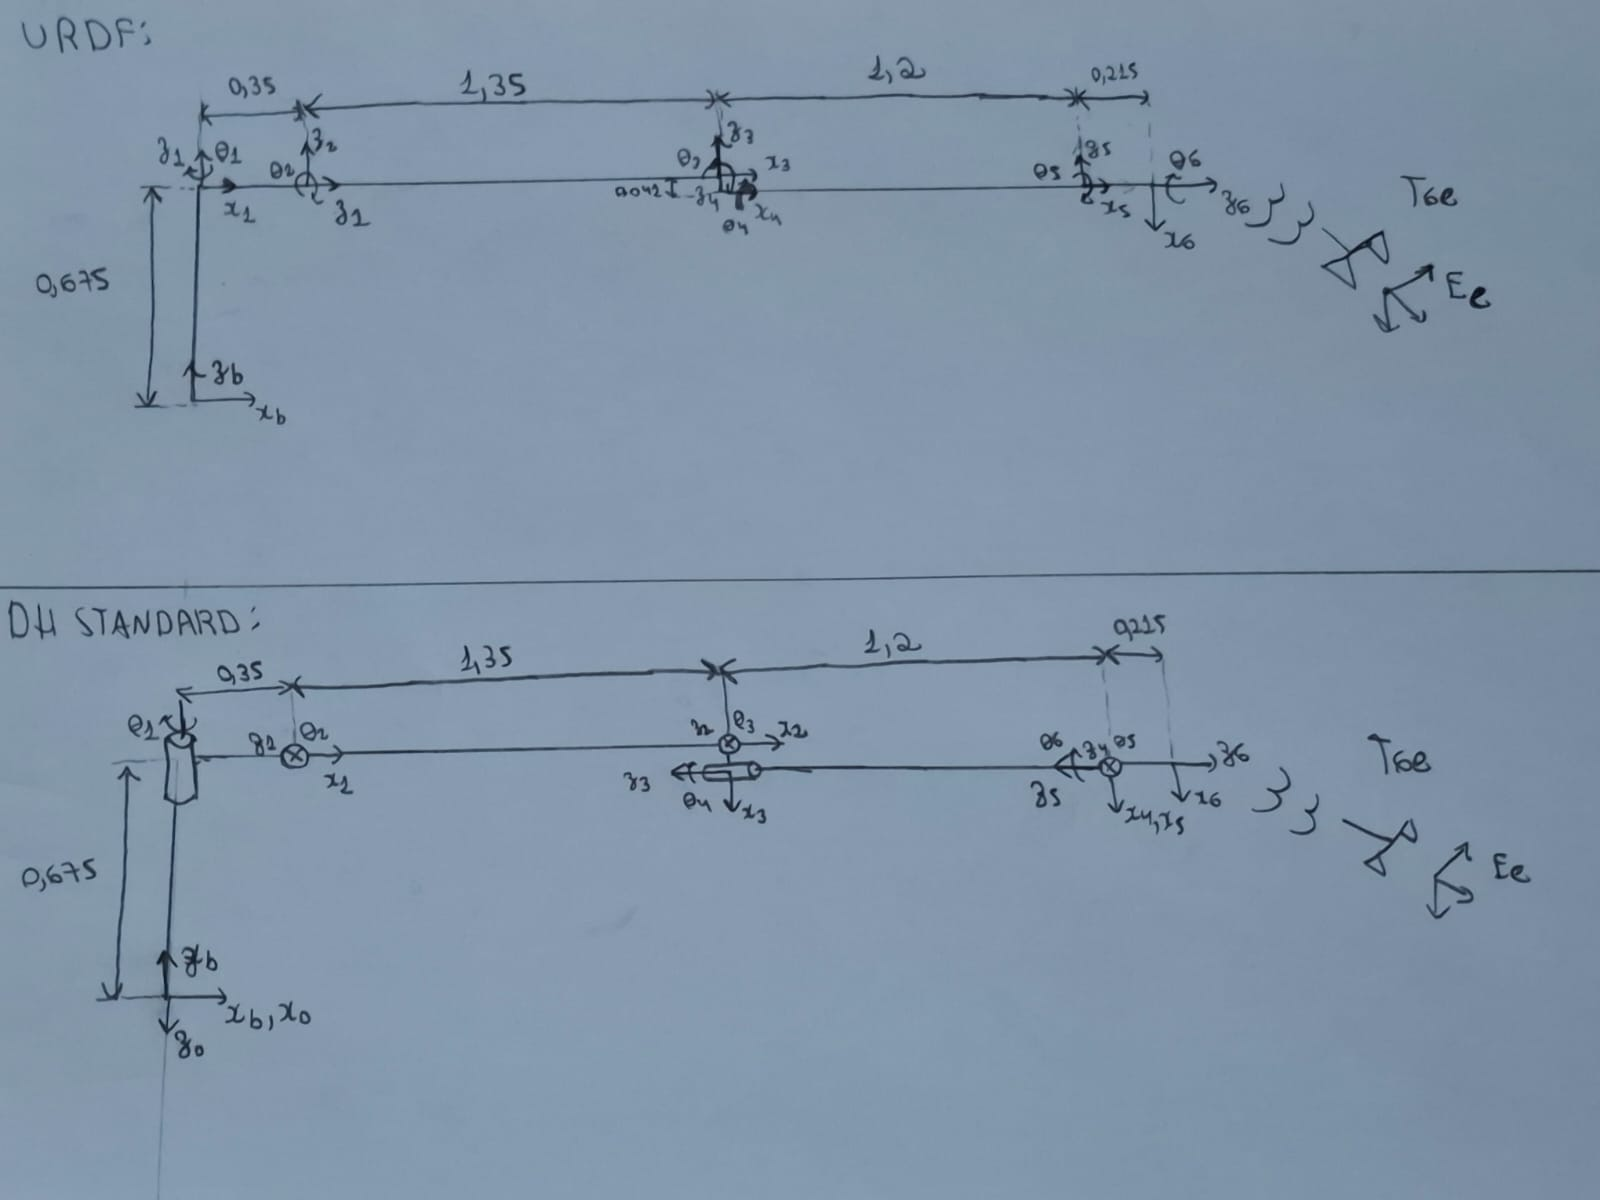
\includegraphics[scale=0.175]{dh_modelo1.jpeg}
    \caption{Diagramas do URDF e DH Standard do braço robótico}
\end{figure}

\subsection{Parâmetros de Denavit-Hartenberg da mesa posicionadora KP2}

\quad Para determinar os parâmetros de Denavit-Hartenberg da mesa posicionadora KP2, foi necessário analisar o URDF dessa mesa posicionadora que pode ser descrita pela seguinte tabela:

\begin{table}[h!]
    \centering
    \begin{tabular}{|c|c|c|c|c|c|c|}
    \hline
    \textbf{Joint $i$} & \textbf{parent} & \textbf{child} & \textbf{xyz} & \textbf{rpy} & \textbf{type} & \textbf{axis} \\ \hline
    1 & kp2\_base\_link & kp2\_link\_1 & 0, 0, 0.865 & 0, 3.1416, 0 & revolute & 1, 0, 0 \\ \hline
    2 & kp2\_link\_1 & kp2\_link\_2 & 0, 0, -0.22 & 0, 3.1416, 0 & revolute & 0, 0, 1 \\ \hline
    3 & kp2\_link\_2 & kp2\_tool0 & 0, 0, 0 & 0, 0, 0 & fixed & - \\ \hline
    \end{tabular}
    \caption{URDF da mesa posicionadora KP2}
\end{table}

\quad Além disso, foi posicionado o eixo z do sistema de coordenadas 0 \((z_0)\) no mesmo sentido e direção do eixo de rotação da junta 1.
Fazendo a seguinte transformação homogênea da base para o eixo de coordenadas 0:

\begin{equation}
    T_{b0} = \begin{bmatrix}
        0 & 0 & -1 & 0 \\
        0 & 1 & 0 & 0 \\
        1 & 0 & 0 & 0.865 \\
        0 & 0 & 0 & 1 
        \end{bmatrix}
\end{equation}

\quad Então, foi possível obter os parâmetros do Denavit-Hartenberg Standard a seguir:

\begin{table}[h!]
    \centering
    \begin{tabular}{|c|c|c|c|c|c|c|}
    \hline
    \textbf{Elo $i$} & $\theta_i$ & $d_i$ & $a_i$ & $\alpha_i$ & \textbf{type} & \textbf{offset} \\ \hline
    1 & $\theta_1$ & 0 & 0 & $-\pi/2$ & revolute & $-\pi/2$ \\ \hline
    2 & $\theta_2$ & 0.22 & 0 & 0 & revolute & $\pi/2$ \\ \hline
    \end{tabular}
    \caption{DH do braço robótico}
\end{table}

\quad Além disso, foi necessário obter a transformação homogênea do sistema de coordenadas 2 para o efetuador a seguir:

\begin{equation}
    T_{2e} = \begin{bmatrix}
        1 & 0 & 0 & 0 \\
        0 & 1 & 0 & 0 \\
        0 & 0 & 1 & 0 \\
        0 & 0 & 0 & 1 
        \end{bmatrix}
\end{equation}

\quad Para obter os parâmetros de Denavit-Hartenberg e as transformações homogêneas acima,
foi seguido os seguintes diagramas:

\begin{figure}[h]
    \centering
    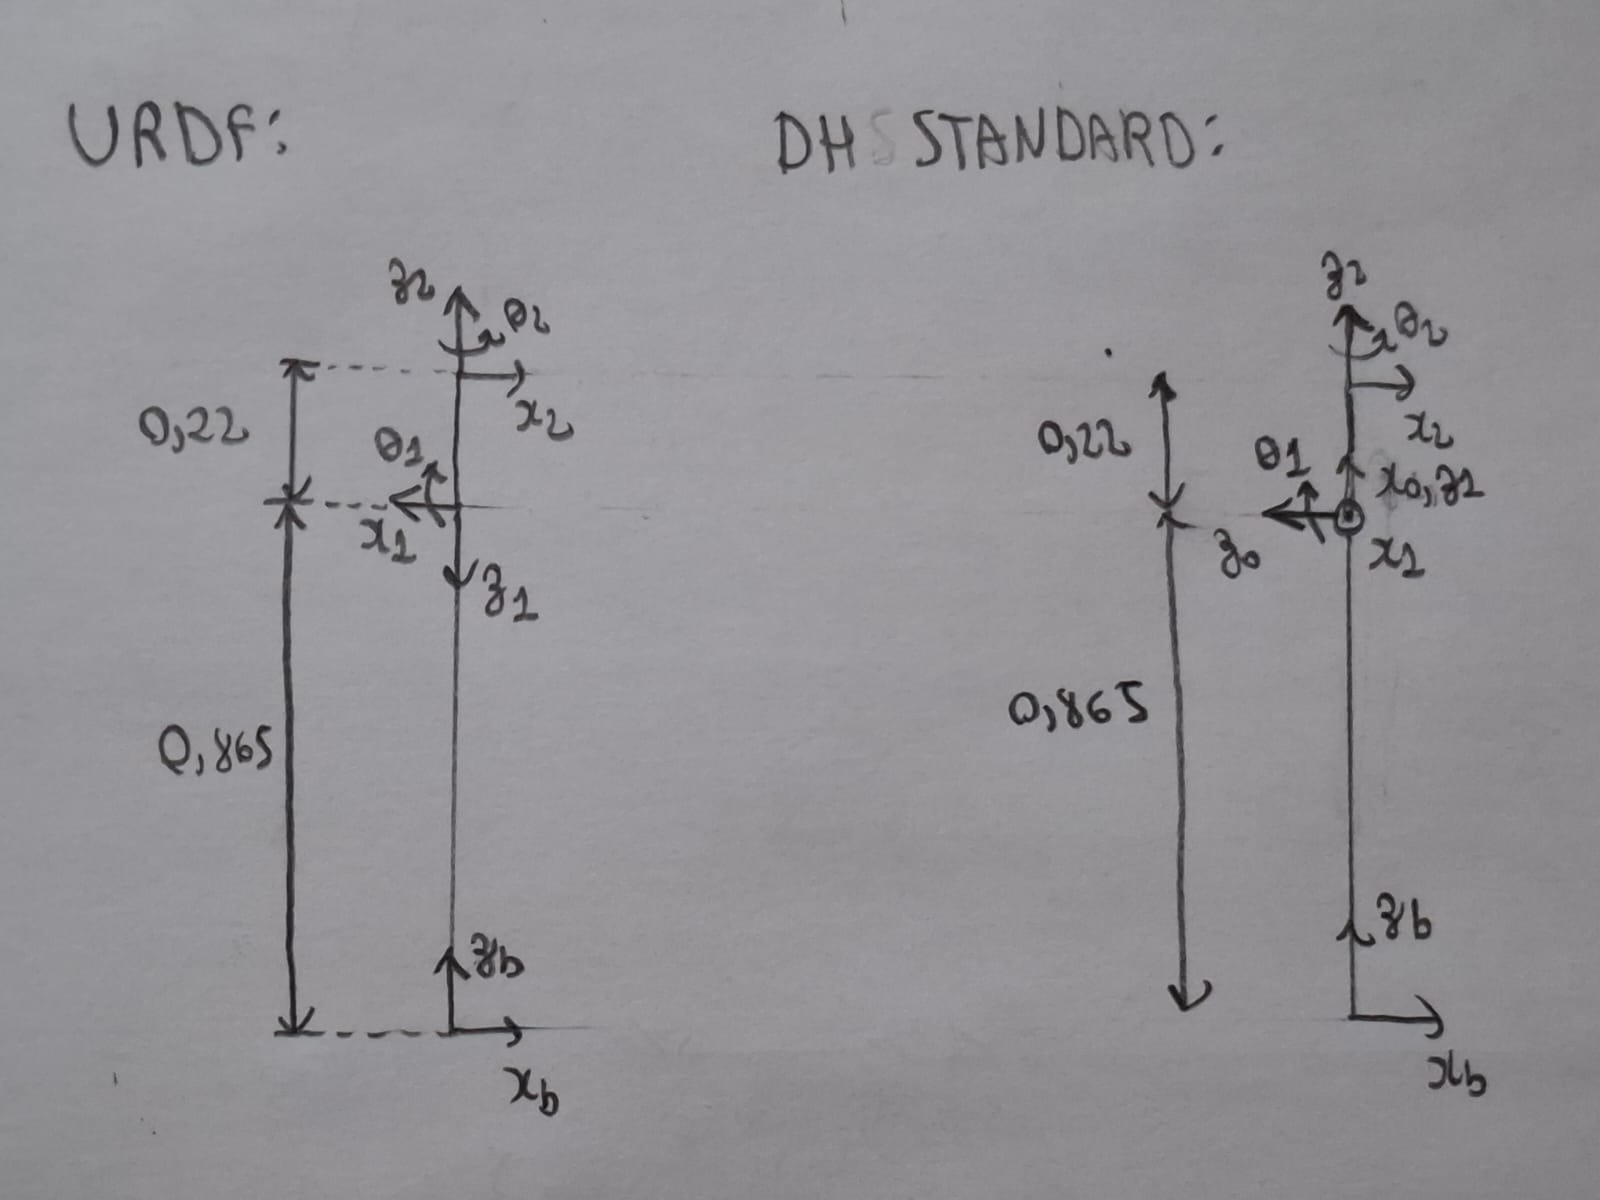
\includegraphics[scale=0.175]{dh_modelo2.jpeg}
    \caption{Diagramas do URDF e DH Standard da mesa posicionadora}
\end{figure}

\subsection{Parâmetros de Denavit-Hartenberg dos sistemas KR90-KP2}

\quad Para determinar os parâmetros de Denavit-Hartenberg do sistema KR90-KP2,
foi necessário analisar o URDF do braço robótico KP90, da mesa posicionadora KP2 e
a transformação homogênea do sistema de coordenadas da mesa $F_{tb}$ com respeito a base do braço $F_{ab}$,
que estão respectivamente na Tabela 1, na Tabela 2 e na fórmula (1).


\quad Além disso, foi posicionado o eixo z do sistema de coordenadas 0 \((z_0)\) no mesmo sentido e direção do eixo de rotação da junta 1.
Fazendo a seguinte transformação homogênea da base para o eixo de coordenadas 0:

\begin{equation}
    T_{b0} = \begin{bmatrix}
        1 & 0 & 0 & 0 \\
        0 & -1 & 0 & 0 \\
        0 & 0 & -1 & 0 \\
        0 & 0 & 0 & 1
        \end{bmatrix}
\end{equation}

\quad Então, foi possível obter os parâmetros do Denavit-Hartenberg Standard a seguir:

\begin{table}[h!]
    \centering
    \begin{tabular}{|c|c|c|c|c|c|c|}
    \hline
    \textbf{Elo $i$} & $\theta_i$ & $d_i$ & $a_i$ & $\alpha_i$ & \textbf{type} & \textbf{offset} \\ \hline
    1 & $\theta_1$ & 0.22 & 0 & $\pi/2$ & revolute & $\pi/2$ \\ \hline
    2 & $\theta_2$ & 1.73923 & -0.39198 & $-\pi/2$ & revolute & 0 \\ \hline
    3 & $\theta_3$ & -0.27360 & 0.35 & $\pi/2$ & revolute & $\pi/2$ \\ \hline
    4 & $\theta_4$ & 0 & 1.35 & 0 & revolute & 0 \\ \hline
    5 & $\theta_5$ & 0 & 0.041 & $-\pi/2$ & revolute & $\pi/2$ \\ \hline
    6 & $\theta_6$ & -1.2 & 0 & $\pi/2$ & revolute & 0 \\ \hline
    7 & $\theta_7$ & 0 & 0 & $-\pi/2$ & revolute & 0 \\ \hline
    8 & $\theta_8$ & -0.215 & 0 & $-\pi$ & revolute & 0 \\ \hline
    \end{tabular}
    \caption{DH do sistema KP90-KP2}
\end{table}

\quad Além disso, foi necessário obter a transformação homogênea do sistema de coordenadas 8 para o efetuador a seguir:

\begin{equation}
    T_{8e} = \begin{bmatrix}
        0.61978941 & -0.09040281 & 0.77954372 & 0.03046 \\
        -0.05855747 & 0.98524594 & 0.16081497 & 0.033 \\
        -0.78258041 & -0.14531952 & 0.60535125 & 0.43161 \\
        0 & 0 & 0 & 1 
        \end{bmatrix}
\end{equation}

\quad Para obter os parâmetros de Denavit-Hartenberg e as transformações homogêneas acima,
foi seguido o seguinte diagrama:

\begin{figure}[h]
    \centering
    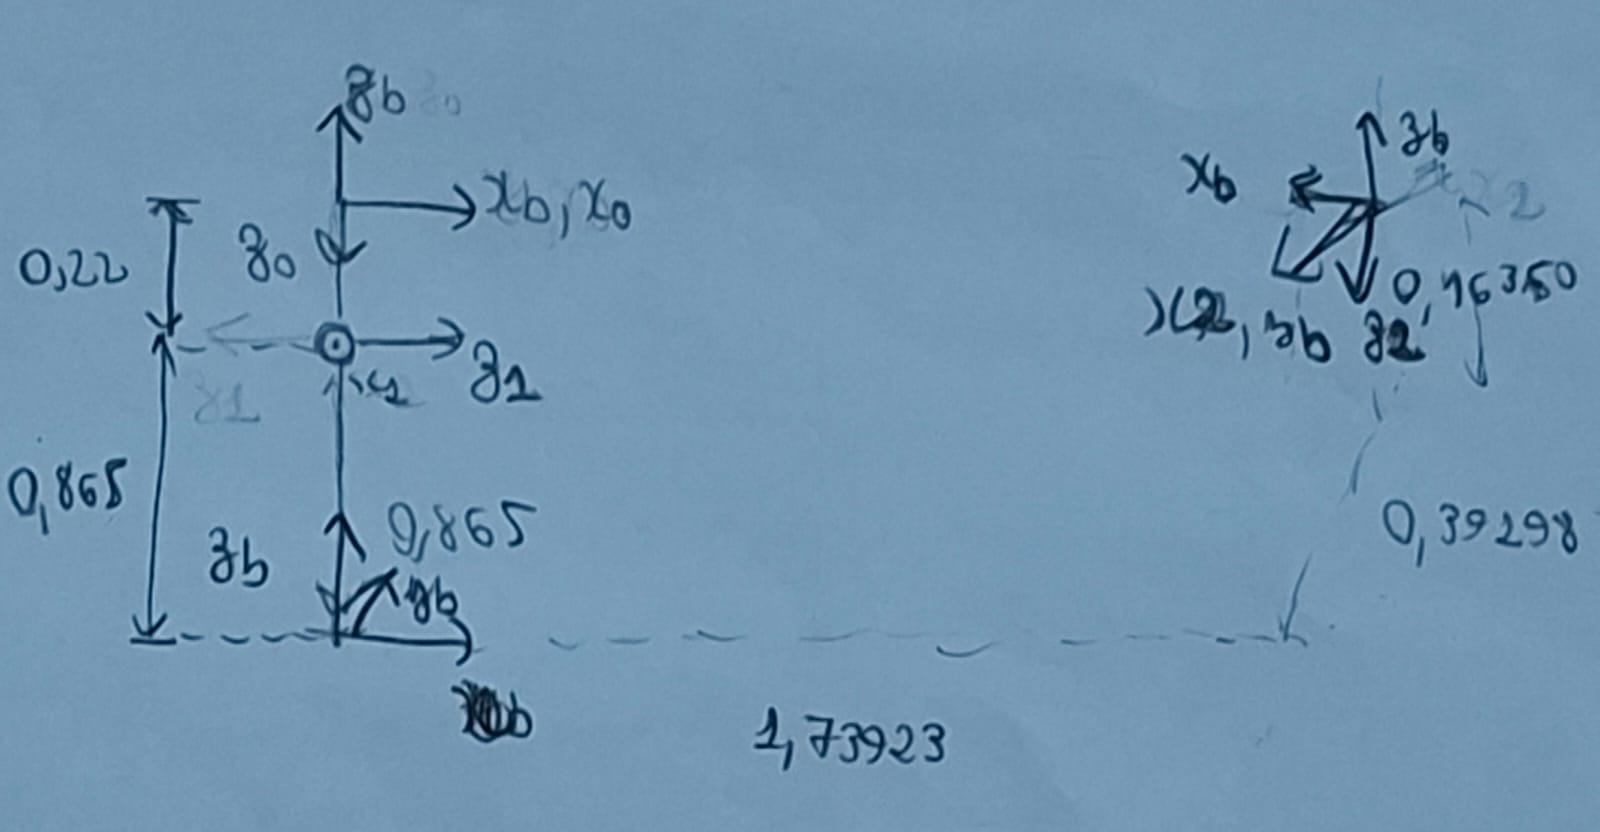
\includegraphics[scale=0.2]{dh_modelo3.jpeg}
    \caption{Diagrama do DH Standard do sistema KR90-KP2}
\end{figure}

\subsection{Modelos dos sistemas}

\quad Utilizando o Robot Toolbox do Matlab foi construído os modelos utilizando a classe SerialLink de cada um dos 3 itens anteriores.
Portanto, para realizar essa construção dos modelos, foi necessário utilizar a transformação homogênea da base para o eixo de coordenadas 0 \( (T_{b0}) \),
o Denavit-Hartenberg do eixo de coordenadas 0 até o eixo de coordenadas do número de juntas \( (T_{0n}) \) e
a transformação homogênea do último eixo de coordenadas do Denavit-Hartenberg até o eixo de coordenadas do efetuador \( (T_{ne}) \).

% Imagem modelo 1
\begin{figure}[h!]
    \centering
    % Modelo 1
    \begin{subfigure}[b]{0.25\textwidth}
        \centering
        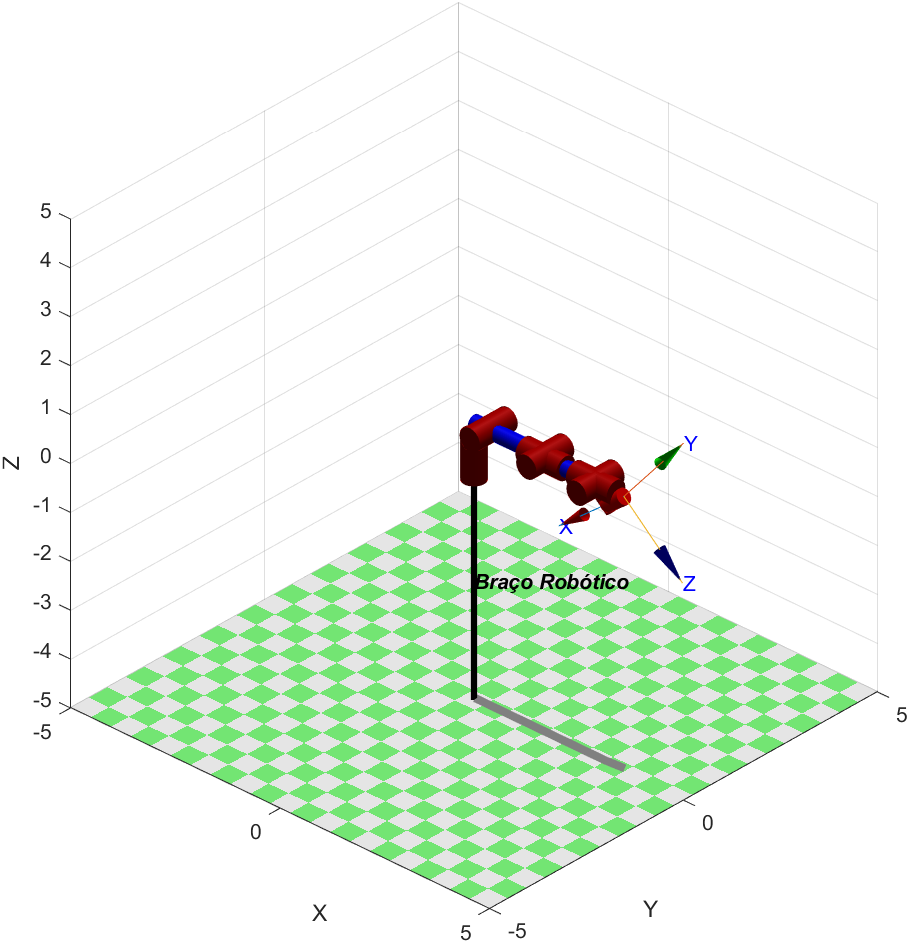
\includegraphics[width=\textwidth]{figura2_modelo_braço.png}
        \caption{Modelo do sistema do braço robótico}
        \label{fig:braço}
    \end{subfigure}
    \hfill
    % Modelo 2
    \begin{subfigure}[b]{0.25\textwidth}
        \centering
        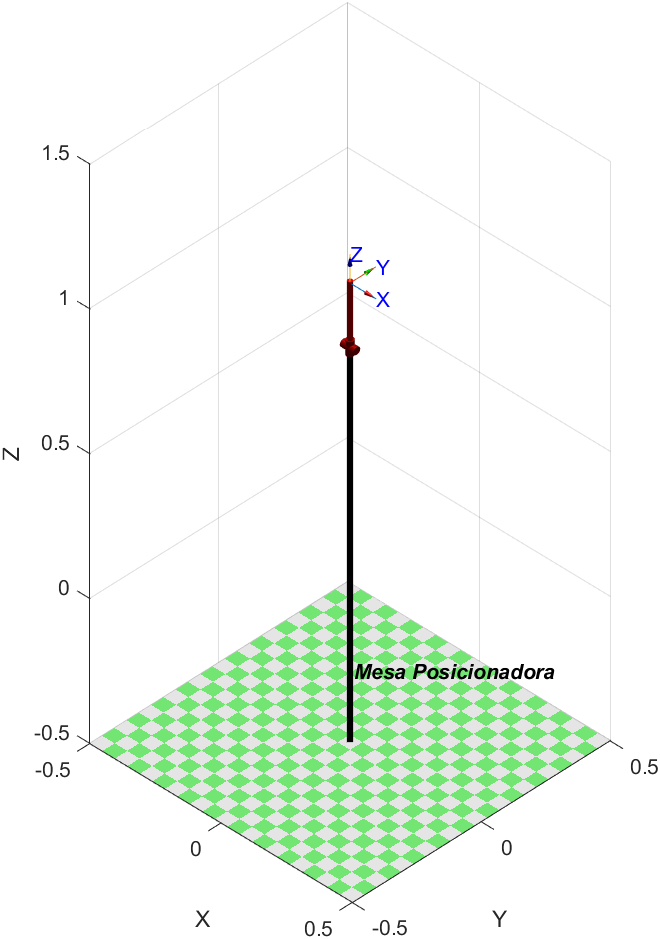
\includegraphics[width=\textwidth]{figura3_modelo_mesa.png}
        \caption{Modelo do sistema da mesa posicionadora}
        \label{fig:mesa}
    \end{subfigure}
    \hfill
    % Modelo 3
    \begin{subfigure}[b]{0.25\textwidth}
        \centering
        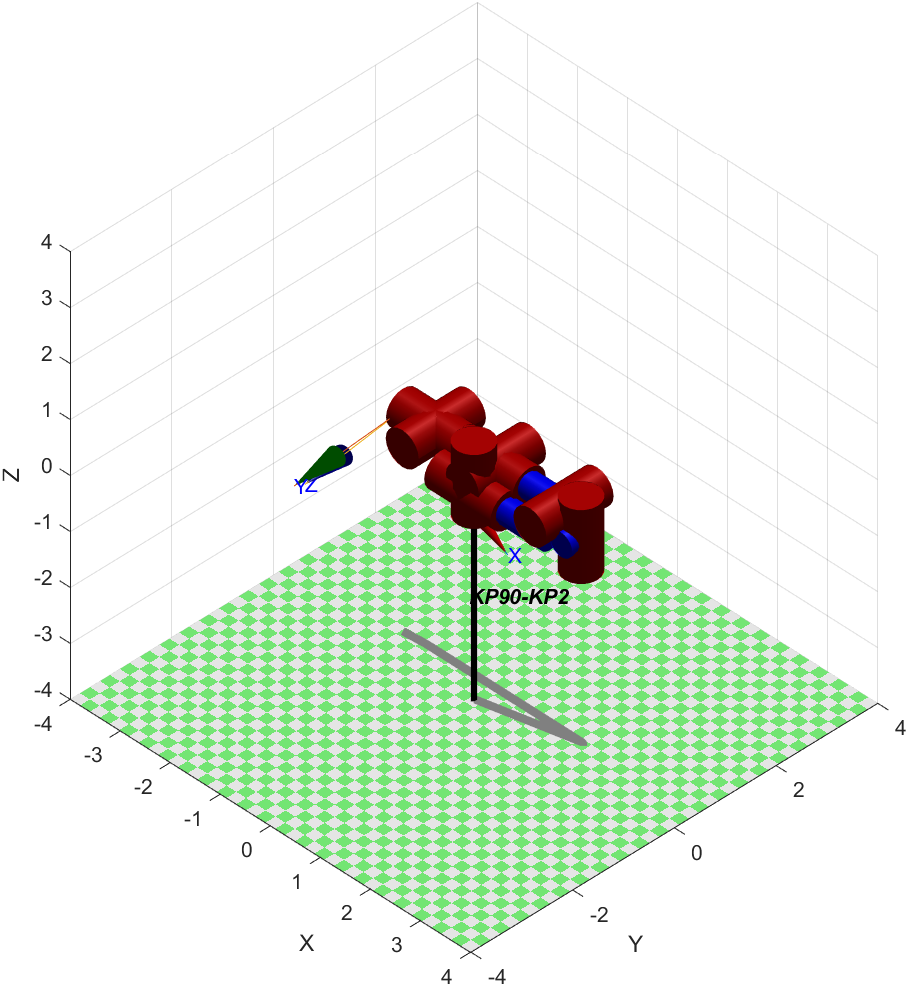
\includegraphics[width=\textwidth]{figura4_modelo_kr90kp2.png}
        \caption{Modelo do sistema KR90-KP2}
        \label{fig:kr90kp2}
    \end{subfigure}
    
    % Legenda geral
    \caption{Modelos dos sistemas analisados. Cada subfigura apresenta um modelo específico utilizado no estudo.}
    \label{fig:modelos}
\end{figure}

\subsection{Validação dos parâmetros de Denavit-Hartenberg}

\quad Foi feita a visualização de 4 configurações diferentes para cada modelo utilizando o Robot Toolbox do Matlab.

% 4 Imagens das configurações do modelo 1
\begin{figure}[h!]
    \centering
    \begin{subfigure}[b]{0.2\textwidth}
        \centering
        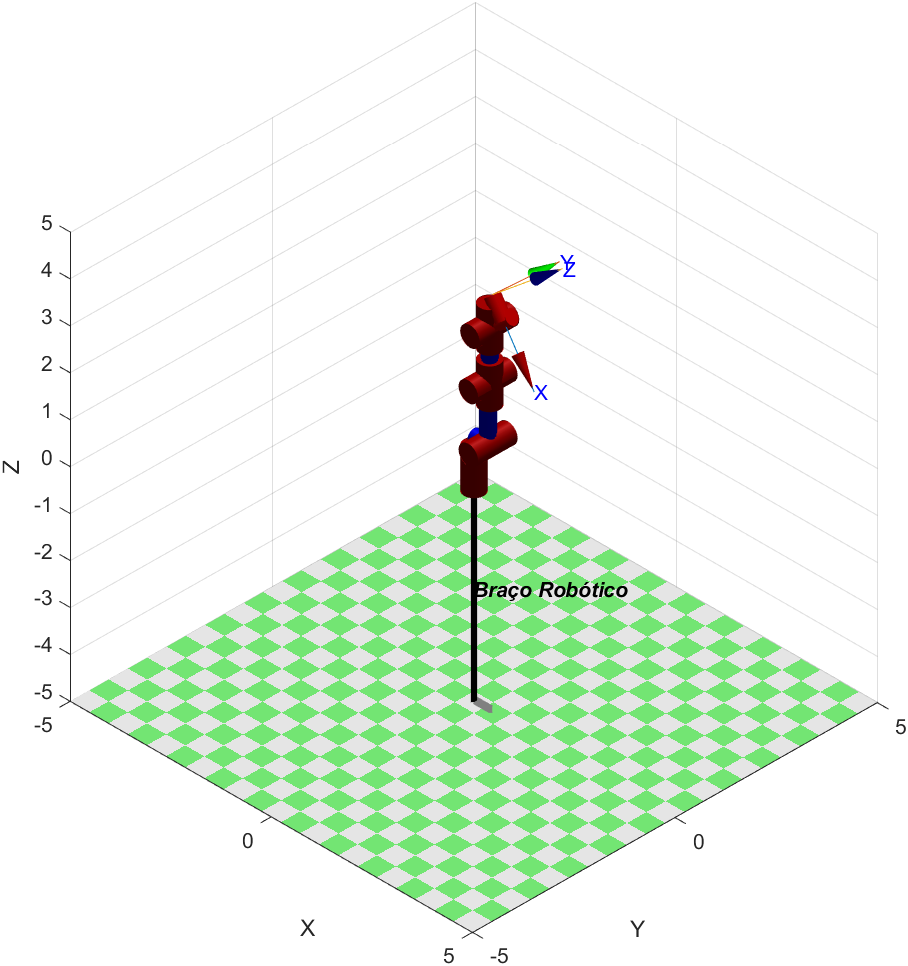
\includegraphics[width=\textwidth]{figura5_modelo1_theta2_minus90.png}
        \caption{$\theta_2 = -90^{\circ}$}
        \label{fig:modelo1_1}
    \end{subfigure}
    \hfill
    \begin{subfigure}[b]{0.2\textwidth}
        \centering
        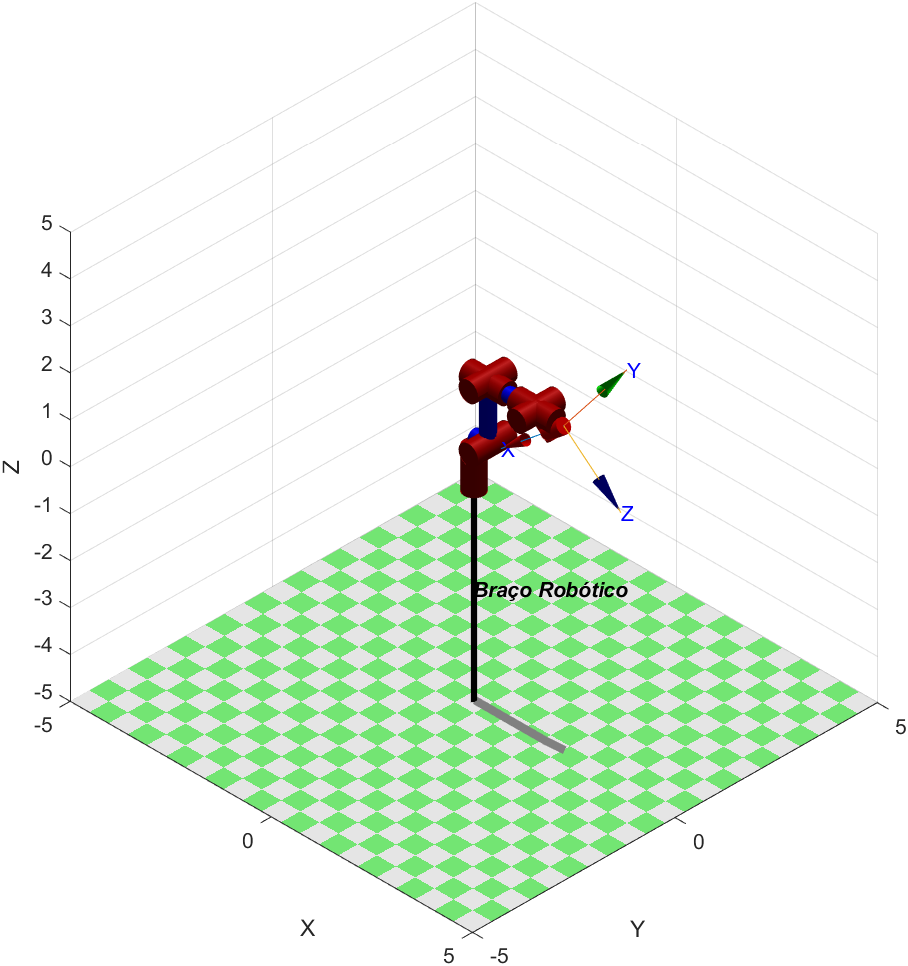
\includegraphics[width=\textwidth]{figura5_modelo1_theta2_minus90_theta3_90.png}
        \caption{$\theta_2 = -90^{\circ}$ e $\theta_3 = 90^{\circ}$}
        \label{fig:modelo1_2}
    \end{subfigure}
    \hfill
    \begin{subfigure}[b]{0.2\textwidth}
        \centering
        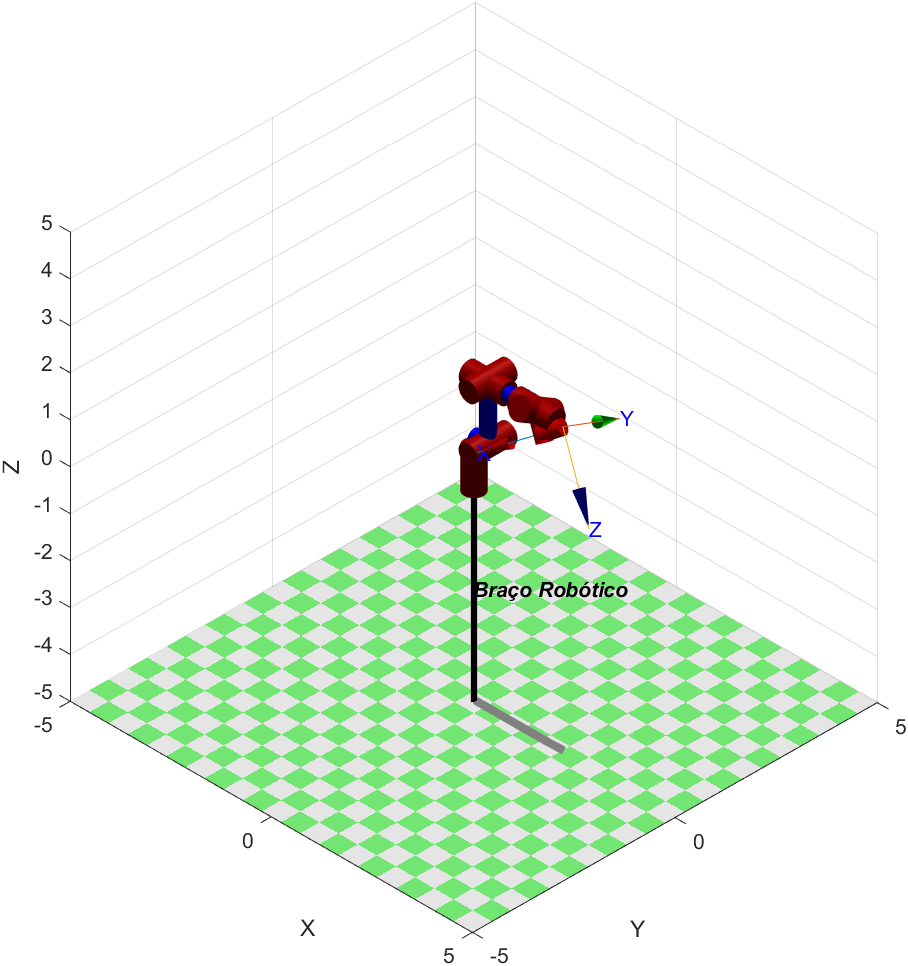
\includegraphics[width=\textwidth]{figura5_modelo1_theta2_minus90_theta3_90_theta4_30.png}
        \caption{$\theta_2 = -90^{\circ}$, $\theta_3 = 90^{\circ}$ e $\theta_4 = 30^{\circ}$}
        \label{fig:modelo1_3}
    \end{subfigure}
    \hfill
    \begin{subfigure}[b]{0.2\textwidth}
        \centering
        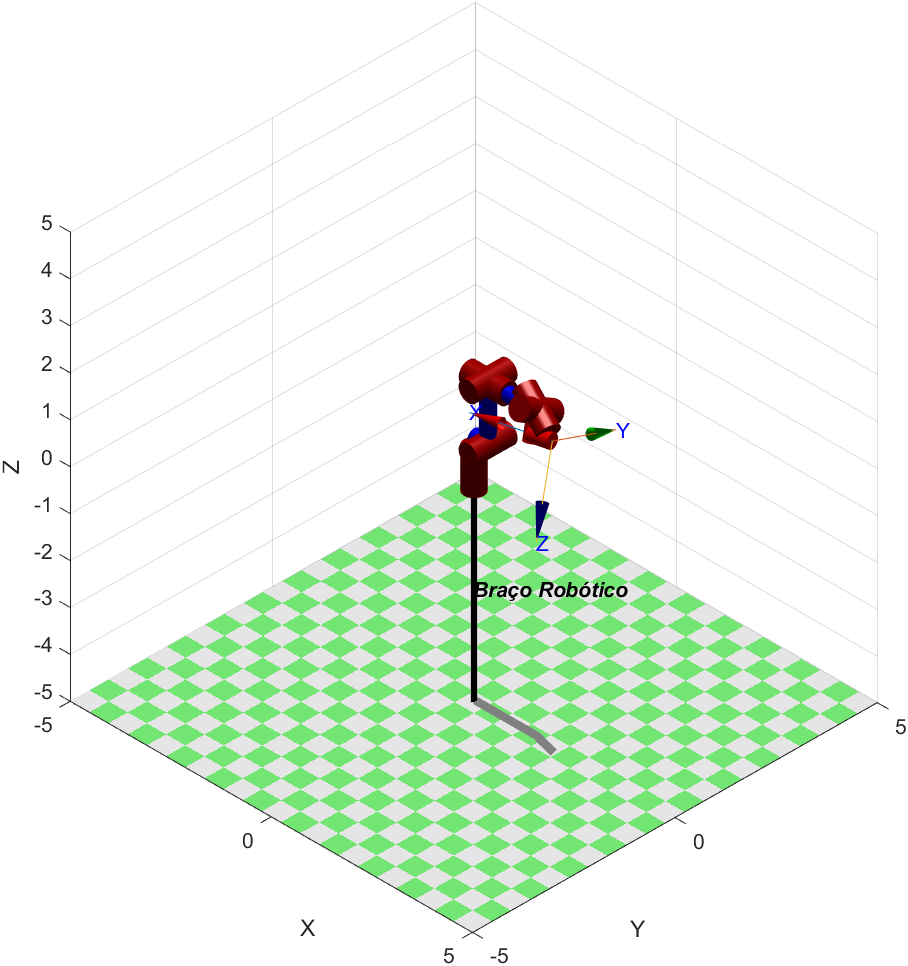
\includegraphics[width=\textwidth]{figura5_modelo1_theta2_minus90_theta3_90_theta4_30_theta5_30.png}
        \caption{$\theta_2 = -90^{\circ}$, $\theta_3 = 90^{\circ}$, $\theta_4 = 30^{\circ}$ e $\theta_5 = 30^{\circ}$}
        \label{fig:modelo1_4}
    \end{subfigure}
    
    % Legenda geral
    \caption{4 configurações diferentes para o modelo do braço robótico.}
    \label{fig:modelos_1}
\end{figure}

% 4 Imagens das configurações do modelo 2
\begin{figure}[h!]
    \centering
    \begin{subfigure}[b]{0.2\textwidth}
        \centering
        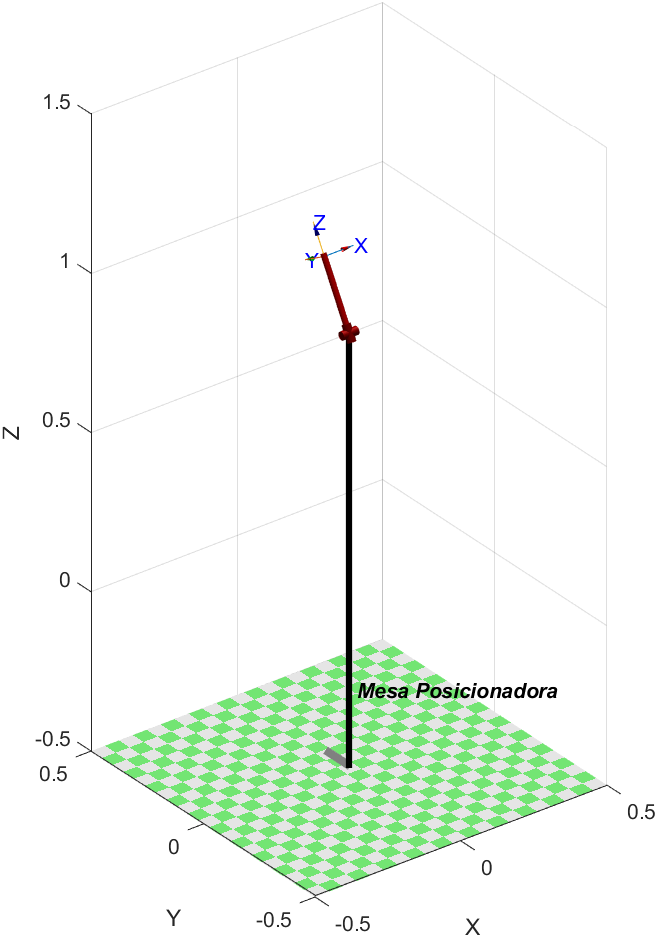
\includegraphics[width=\textwidth]{figura6_modelo2_theta1_30.png}
        \caption{$\theta_1 = 30^{\circ}$}
        \label{fig:modelo2_1}
    \end{subfigure}
    \hfill
    \begin{subfigure}[b]{0.2\textwidth}
        \centering
        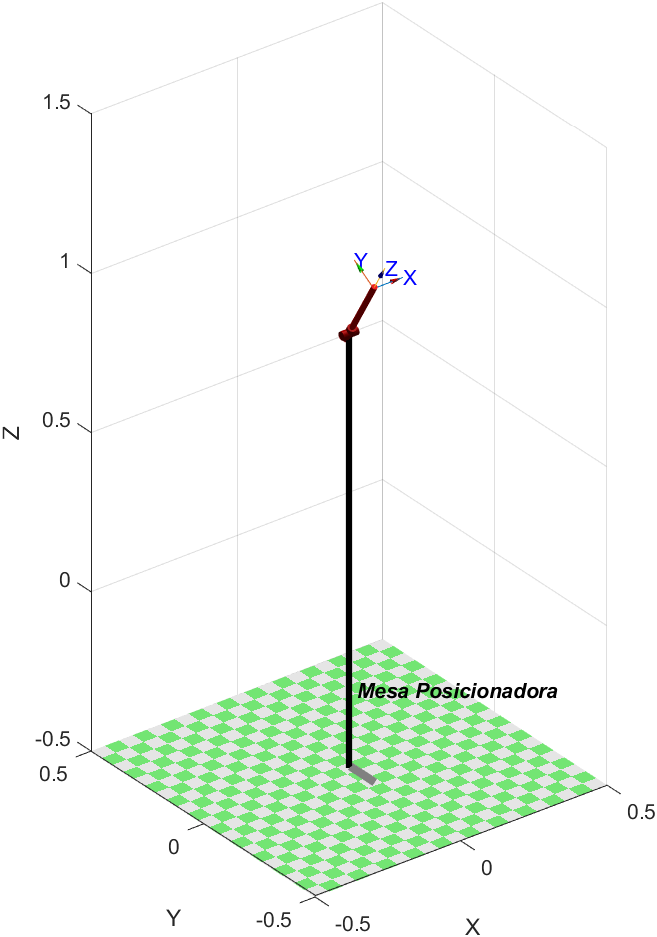
\includegraphics[width=\textwidth]{figura6_modelo2_theta1_minus30.png}
        \caption{$\theta_1 = -30^{\circ}$}
        \label{fig:modelo2_2}
    \end{subfigure}
    \hfill
    \begin{subfigure}[b]{0.2\textwidth}
        \centering
        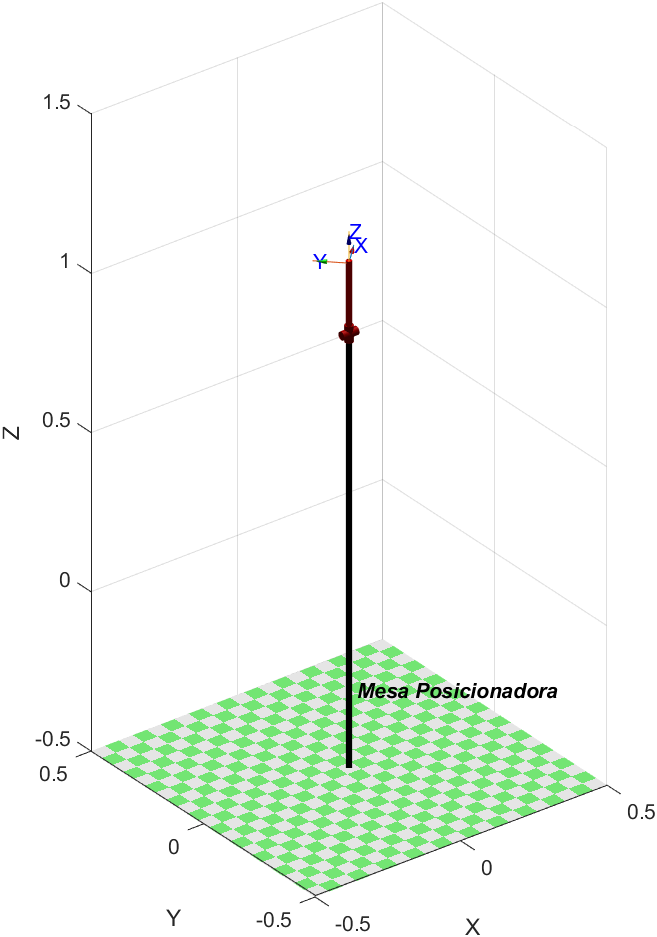
\includegraphics[width=\textwidth]{figura6_modelo2_theta2_45.png}
        \caption{$\theta_2 = 45^{\circ}$}
        \label{fig:modelo2_3}
    \end{subfigure}
    \hfill
    \begin{subfigure}[b]{0.2\textwidth}
        \centering
        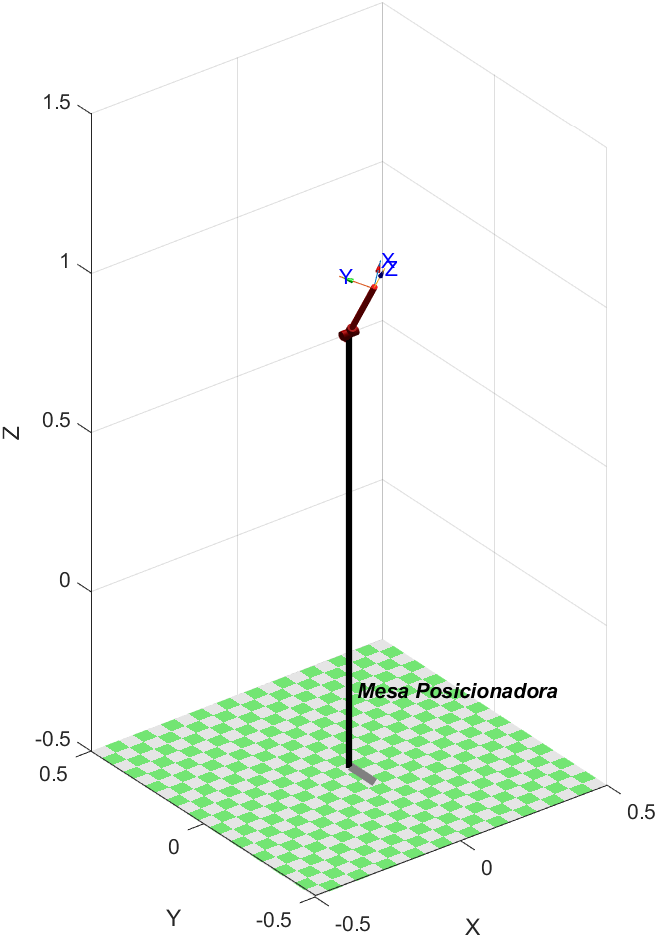
\includegraphics[width=\textwidth]{figura6_modelo2_theta1_minus30_theta2_45.png}
        \caption{$\theta_1 = -30^{\circ}$ e $\theta_2 = 45^{\circ}$}
        \label{fig:modelo2_4}
    \end{subfigure}
    
    % Legenda geral
    \caption{4 configurações diferentes para o modelo da mesa posicionadora.}
    \label{fig:modelos_2}
\end{figure}
% 4 Imagens das configurações do modelo 3
\begin{figure}[h!]
    \centering
    \begin{subfigure}[b]{0.2\textwidth}
        \centering
        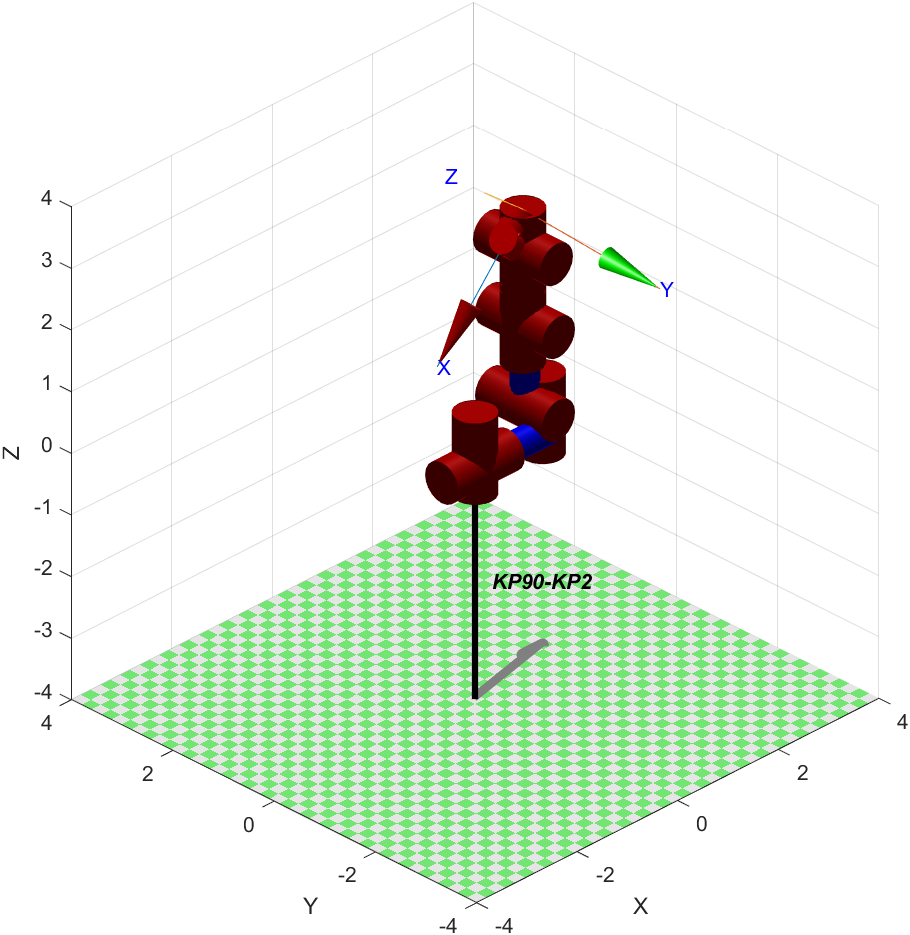
\includegraphics[width=\textwidth]{figura7_modelo3_theta4_minus90.png}
        \caption{$\theta_4 = -90^{\circ}$}
        \label{fig:modelo3_1}
    \end{subfigure}
    \hfill
    \begin{subfigure}[b]{0.2\textwidth}
        \centering
        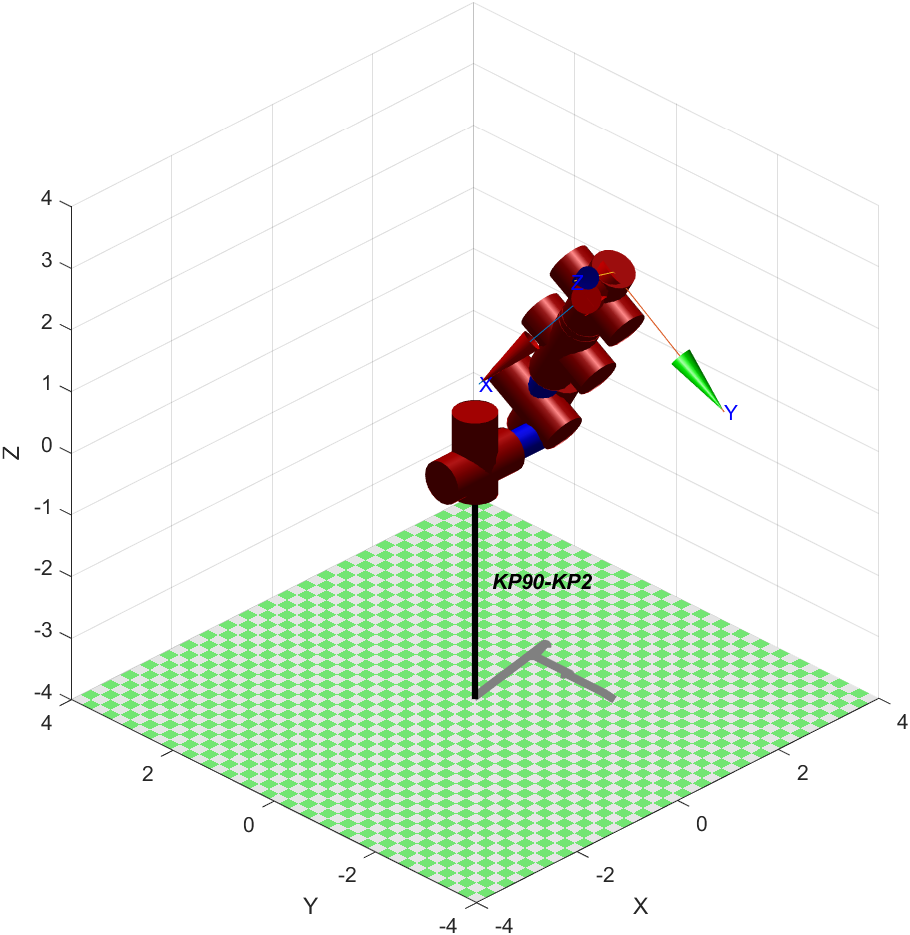
\includegraphics[width=\textwidth]{figura7_modelo3_theta4_minus90_theta2_30.png}
        \caption{$\theta_2 = 30^{\circ}$ e $\theta_4 = -90^{\circ}$}
        \label{fig:modelo3_2}
    \end{subfigure}
    \hfill
    \begin{subfigure}[b]{0.2\textwidth}
        \centering
        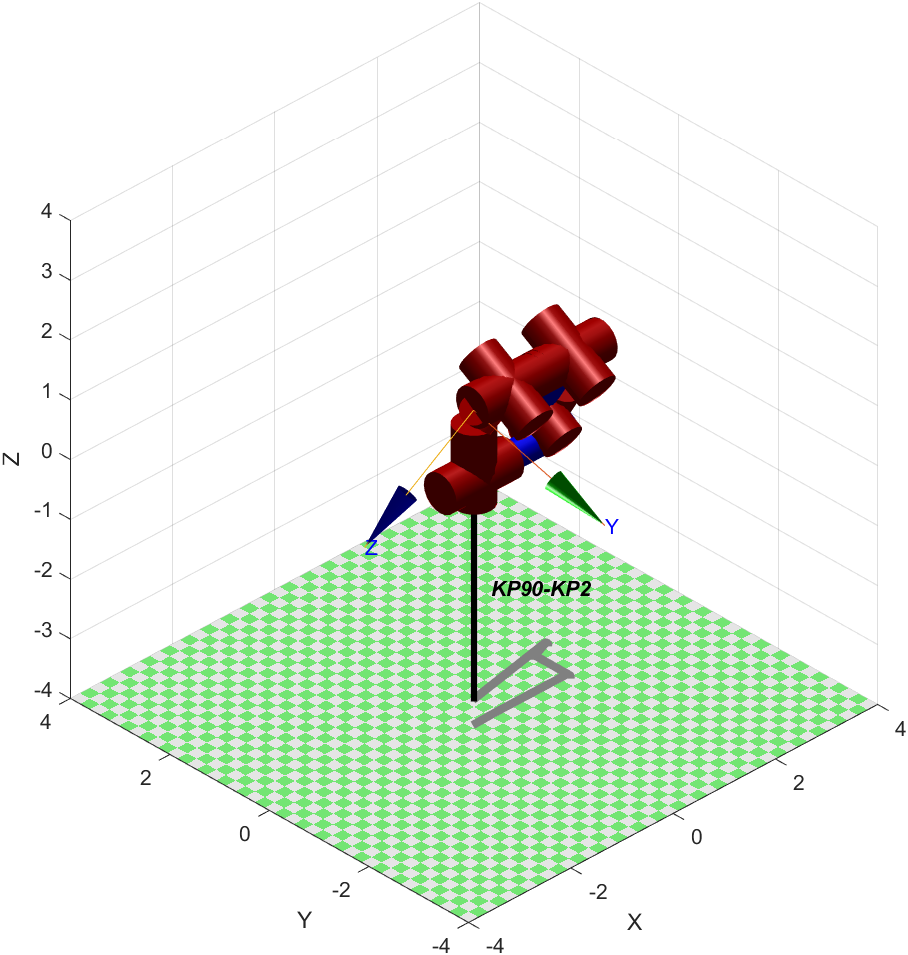
\includegraphics[width=\textwidth]{figura7_modelo3_theta4_minus90_theta2_30_theta5_90.png}
        \caption{$\theta_2 = 30^{\circ}$, $\theta_4 = -90^{\circ}$ e $\theta_5 = 90^{\circ}$}
        \label{fig:modelo3_3}
    \end{subfigure}
    \hfill
    \begin{subfigure}[b]{0.2\textwidth}
        \centering
        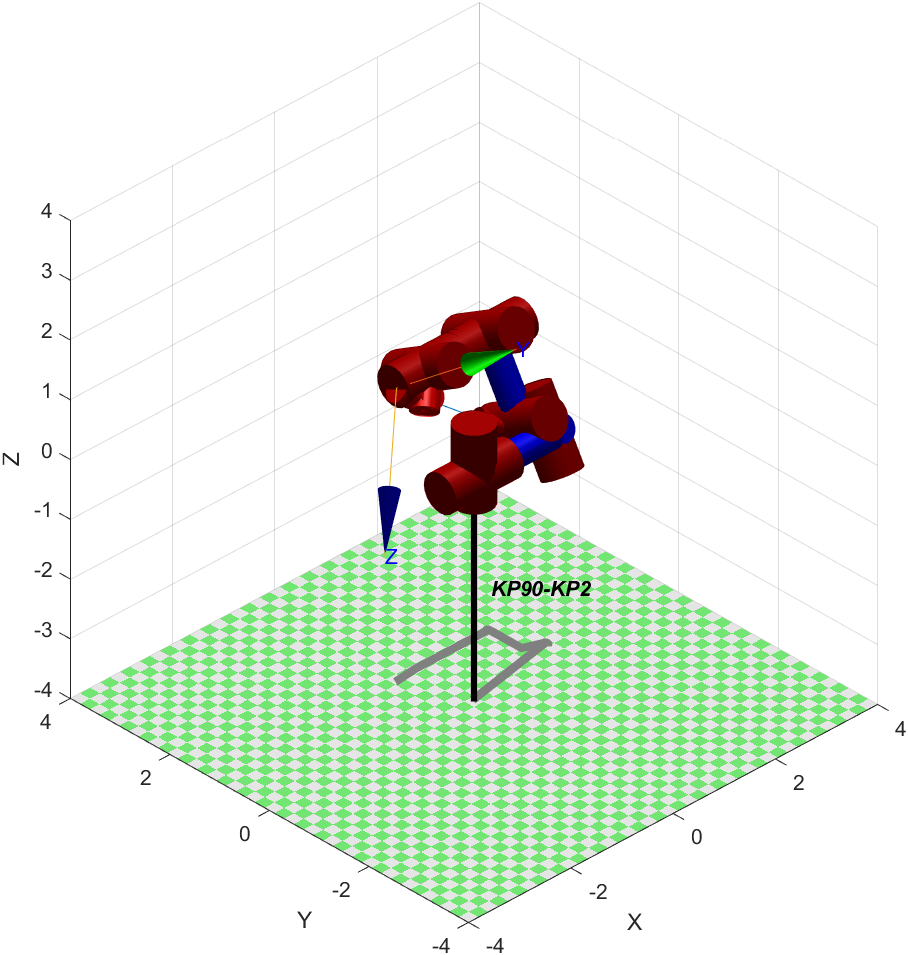
\includegraphics[width=\textwidth]{figura7_modelo3_theta4_minus90_theta2_minus30_theta5_90.png}
        \caption{$\theta_2 = -30^{\circ}$, $\theta_4 = -90^{\circ}$ e $\theta_5 = 90^{\circ}$}
        \label{fig:modelo3_4}
    \end{subfigure}
    
    % Legenda geral
    \caption{4 configurações diferentes para o modelo do sistema KR90-KP2.}
    \label{fig:modelos_3}
\end{figure}

\subsection{Verificação dos resultados da cinemática inversa}

\quad Neste estudo, foi explorado a função \texttt{ikine()} da \textit{Robotics Toolbox} para calcular a cinemática inversa do robô serial \texttt{Kr90}, considerando uma trajetória em zigue-zague para o efetuador $F_t$ em relação ao referencial $F_{de}$. Os \textit{waypoints} utilizados são apresentados na Tabela~\ref{tab:waypoints}. A orientação foi mantida constante para todos os casos, definida pelos ângulos de \textit{roll} $= \pi$, \textit{pitch} $= 0$ e \textit{yaw} $= \pi/2$. Além disso, os ângulos das juntas da mesa posicionadora foram fixados em $\boldsymbol{\theta_t} = [\pi/4, 0]$.

\begin{table}[h!]
    \centering
    \begin{tabular}{|c|c|}
    \hline
    \textbf{Waypoint} & \textbf{Posição $\boldsymbol{p_{dt}}$ (m)} \\ \hline
    1                 & $[0.04, 0, 0]^T$                          \\ \hline
    2                 & $[-0.04, 0, 0]^T$                         \\ \hline
    3                 & $[-0.04, 0.01, 0]^T$                      \\ \hline
    4                 & $[0.04, 0.01, 0]^T$                       \\ \hline
    5                 & $[0.04, 0.02, 0]^T$                       \\ \hline
    6                 & $[-0.04, 0.02, 0]^T$                      \\ \hline
    7                 & $[-0.04, 0.03, 0]^T$                      \\ \hline
    8                 & $[0.04, 0.03, 0]^T$                       \\ \hline
    9                 & $[0.04, 0.04, 0]^T$                       \\ \hline
    10                & $[-0.04, 0.04, 0]^T$                      \\ \hline
    \end{tabular}
    \caption{\textit{Waypoints} da trajetória em zigue-zague.}
    \label{tab:waypoints}
\end{table}


\quad Os parâmetros da função \texttt{ikine()} foram explorados para cada \textit{waypoint}, ajustando-se tolerância (\texttt{tol}), ângulos iniciais (\texttt{q0}), fator de amortecimento (\texttt{lambda}) e máscara de restrições (\texttt{mask}). Os resultados obtidos são apresentados a seguir:

\begin{table}[h!]
    \centering
    \begin{tabular}{|c|c|c|c|c|c|c|}
    \hline
    \textbf{Waypoint} & $\boldsymbol{\theta_1}$ & $\boldsymbol{\theta_2}$ & $\boldsymbol{\theta_3}$ & $\boldsymbol{\theta_4}$ & $\boldsymbol{\theta_5}$ & $\boldsymbol{\theta_6}$ \\ \hline
    1 & 0.2438 & -0.7993 & 2.0019 & 1.6157 & -1.7229 & -0.2979 \\ \hline
    2 & 0.2329 & -0.7770 & 1.9295 & 1.5979 & -1.7205 & -0.3488 \\ \hline
    3 & 0.2368 & -0.7713 & 1.9271 & 1.6020 & -1.7219 & -0.3453 \\ \hline
    4 & 0.2479 & -0.7933 & 1.9995 & 1.6200 & -1.7241 & -0.2942 \\ \hline
    5 & 0.2519 & -0.7873 & 1.9971 & 1.6244 & -1.7254 & -0.2906 \\ \hline
    6 & 0.2406 & -0.7655 & 1.9247 & 1.6061 & -1.7234 & -0.3419 \\ \hline
    7 & 0.2445 & -0.7598 & 1.9222 & 1.6102 & -1.7248 & -0.3385 \\ \hline
    8 & 0.2560 & -0.7813 & 1.9945 & 1.6287 & -1.7266 & -0.2870 \\ \hline
    9 & 0.2600 & -0.7753 & 1.9919 & 1.6331 & -1.7278 & -0.2835 \\ \hline
    10 & 0.2484 & -0.7540 & 1.9197 & 1.6142 & -1.7262 & -0.3352 \\ \hline
    \end{tabular}
    \caption{Valores dos ângulos das juntas ($\theta_1$ a $\theta_6$) para cada \textit{waypoint}.}
    \label{tab:theta_values}
\end{table}
    

\subsection{Determinação do Jacobiano de $F_t$ com respeito a $F_{de}$}

\subsection{Validação do Jacobiano  de $F_t$ com respeito a $F_{de}$}

\subsection{Implementação da solução da cinemática inversa pelo método iterativo}

\section{Conclusão}

\newpage

\section*{Apêndice}

\begin{lstlisting}[caption={Código do braço robótico (KR90)}, label={code:kr90}]
% Parâmetros DH do robô
L1 = Revolute('d', -0.675, 'a', 0.35, 'alpha', pi/2, 'offset', 0);      % Elo 1
L2 = Revolute('d', 0, 'a', 1.35, 'alpha', 0, 'offset', 0);              % Elo 2
L3 = Revolute('d', 0, 'a', 0.041, 'alpha', -pi/2, 'offset', pi/2);      % Elo 3
L4 = Revolute('d', -1.2, 'a', 0, 'alpha', pi/2, 'offset', 0);           % Elo 4
L5 = Revolute('d', 0, 'a', 0, 'alpha', -pi/2, 'offset', 0);             % Elo 5
L6 = Revolute('d', -0.215, 'a', 0, 'alpha', -pi, 'offset', 0);          % Elo 6

% Definir o robô
robot = SerialLink([L1 L2 L3 L4 L5 L6], 'name', 'Braço Robotico');

% Transformação homogênea da base para o eixo 0 (T_b0)
T_b0 = [1,  0,  0,  0;
        0, -1,  0,  0;
        0,  0, -1,  0;
        0,  0,  0,  1];

T_6e = transl(0.03046, 0.033, 0.43161) * trotz(-5.4) * troty(51.5) * trotx(-13.5);

% Incorporar as transformaçoes no robô
robot.base = SE3(T_b0);  % Define a base do robô
robot.tool = T_6e;  % Define a ferramenta (tool) do robô

% Configuração inicial das juntas (todas em zero)
q0 = zeros(1, 6);

% Calcular a transformação homogênea do efetuador em relação à base (T_be)
T_be = robot.fkine(q0);

% Exibir a transformação final do efetuador
disp('Transformação do efetuador em relação à base (T_be):');
disp(T_be.T);

% Plotar o robô na configuração inicial com controles interativos
figure;
robot.teach(q0, 'workspace', [-5 5 -5 5 -5 5]);
\end{lstlisting}

\newpage

\begin{lstlisting}[caption={Código da mesa poscionadora (KP2)}, label={code:kp2}]
% Parâmetros DH do robô
L1 = Revolute('d', 0, 'a', 0, 'alpha', -pi/2, 'offset', -pi/2);   % Elo 1
L2 = Revolute('d', 0.22, 'a', 0, 'alpha', 0, 'offset', pi/2);     % Elo 2

% Definir o robô
robot = SerialLink([L1 L2], 'name', 'Mesa Posicionadora');

% Transformação homogênea da base para o eixo 0 (T_b0)
T_b0 = [0,  0, -1,  0;
        0,  1,  0,  0;
        1,  0,  0,  0.865;
        0,  0,  0,  1];

% Transformação homogênea do eixo 2 para o efetuador (T_2e)
T_2e = eye(4); % Matriz identidade, conforme especificado

% Incorporar as transformaçoes no robô
robot.base = SE3(T_b0);  % Define a base do robô
robot.tool = SE3(T_2e);  % Define a ferramenta (tool) do robô

% Configuração inicial das juntas (todas em zero)
q0 = zeros(1, 2);

% Calcular a transformação homogênea do efetuador em relação à base (T_be)
T_be = robot.fkine(q0);

% Exibir as transformaçoes
disp('Transformação da base para o efetuador (T_be):');
disp(T_be.T);

% Plotar o robô na configuração inicial com controles interativos
figure;
robot.teach(q0, 'workspace', [-0.5 0.5 -0.5 0.5 -0.5 1.5]);    
\end{lstlisting}

\newpage

\begin{lstlisting}[caption={Código do sistema (KR90-KP2)}, label={code:kr90kp2}]
% Parâmetros DH do sistema KP90-KP2
L1 = Revolute('d', 0.22, 'a', 0, 'alpha', pi/2, 'offset', pi/2);          % Elo 1
L2 = Revolute('d', 1.73923, 'a', -0.39198, 'alpha', -pi/2, 'offset', 0);  % Elo 2
L3 = Revolute('d', -0.27360, 'a', 0.35, 'alpha', pi/2, 'offset', pi/2);   % Elo 3
L4 = Revolute('d', 0, 'a', 1.35, 'alpha', 0, 'offset', 0);                % Elo 4
L5 = Revolute('d', 0, 'a', 0.041, 'alpha', -pi/2, 'offset', pi/2);        % Elo 5
L6 = Revolute('d', -1.2, 'a', 0, 'alpha', pi/2, 'offset', 0);             % Elo 6
L7 = Revolute('d', 0, 'a', 0, 'alpha', -pi/2, 'offset', 0);               % Elo 5
L8 = Revolute('d', -0.215, 'a', 0, 'alpha', -pi, 'offset', 0);            % Elo 6

% Definir o robô
robot = SerialLink([L1 L2 L3 L4 L5 L6 L7 L8], 'name', 'KP90-KP2');

T_8e = transl(0.03046, 0.033, 0.43161) * trotz(-5.4) * troty(51.5) * trotx(-13.5);

% Incorporar as transformaçoes no robô
robot.base = trotx(180);  % Define a base do robô
robot.tool = T_8e;  % Define a ferramenta (tool) do robô

% Configuração inicial das juntas (todas em zero)
q0 = zeros(1, 8);

% Calcular a transformação homogênea do efetuador em relação à base (T_be)
T_be = robot.fkine(q0);

% Exibir as transformaçoes
disp('Transformação da base para o efetuador (T_be):');
disp(T_be.T);

% Plotar o robô na configuração inicial com controles interativos
figure;
robot.teach(q0, 'workspace', [-4 4 -4 4 -4 4]);
\end{lstlisting}

\newpage

\begin{lstlisting}[caption={Código da subseção 2.6}, label={code:subsecao26}]
% Configuração dos Waypoints
waypoints = [ 0.04,  0.00, 0.0; -0.04,  0.00, 0.0; -0.04,  0.01, 0.0; 0.04,  0.01, 0.0; 0.04,  0.02, 0.0;
    -0.04,  0.02, 0.0; -0.04,  0.03, 0.0; 0.04,  0.03, 0.0; 0.04,  0.04, 0.0; -0.04,  0.04, 0.0;];
% ------------------ Configuração do Robô Kuka KR90 ------------------------
% ---------------- Configuração do Robô Kuka KP2 (Mesa Posicionadora) -----------------
% ------------------ Configuração da Transformação entre Robôs -----------------------
% Transformação entre as bases dos robôs
T_Fab_Ftb = SE3;
T_Fab_Ftb.t = [1.73923, 0.39198, -0.46360]; % Translação
T_Fab_Ftb = T_Fab_Ftb * SE3.Rz(180);       % Rotação de 180 graus em Z

% Angulos conhecidos da mesa posicionadora
theta_t = [pi/4, 0]; 
T_Ftb_Fde = robot_kukaKp2.fkine(theta_t); % Cinemática direta do KP2
% ------------------ Cálculo da Cinemática Inversa e Trajetoria -----------------------
% Configuraçoes iniciais
q0 = zeros(1, robot_kukaKr90.n); % Angulos iniciais das juntas
tol = 1e-6;                % Tolerância para solução da cinemática inversa
lambda = 0.1;              % Taxa de regularização

% Matriz para armazenar as soluçoes das juntas
q_solutions = zeros(size(waypoints, 1), robot_kukaKr90.n);

% Iteração para cada waypoint
for i = 1:size(waypoints, 1)
    % Define a transformação desejada para o waypoint atual
    T_Fde_Ft = SE3.Rz(90) * SE3.Rx(180); % Orientação fixa
    T_Fde_Ft.t = waypoints(i, :);        % Posição do waypoint
    
    % Transformação total em relação a base absoluta
    T_Fab_Ft = T_Fab_Ftb * T_Ftb_Fde * T_Fde_Ft;
    
    % Calcula a cinemática inversa
    q_solutions(i, :) = robot_kukaKr90.ikine(T_Fab_Ft, q0, 'tol', tol, 'lambda', lambda, 'mask', [1 1 1 1 1 1]);
    
    % Valida a solução obtida com a cinemática direta
    T_check = robot_kukaKr90.fkine(q_solutions(i, :));
    disp(['Waypoint ', num2str(i)]);
    disp('Transformação homogênea obtida:');
    disp(robot_kukakr90kp2.fkine([0, pi/4, q_solutions(i,:)]));
    disp('Angulos das juntas:');
    disp(q_solutions(i, :));
end
\end{lstlisting}

\end{document}